\documentclass[12pt,a4paper]{article}

\usepackage[T1,T2A]{fontenc}
\usepackage[utf8]{inputenc}
\usepackage[russian]{babel}

\usepackage{indentfirst}
\usepackage[a4paper,top=2cm,bottom=2cm,left=2.5cm,right=1.5cm,marginparwidth=1.75cm]{geometry}
% \linespread{1.5}

\usepackage{titlesec}
% \titleformat{\section}[hang]{\bfseries}{\thesection.}{1em}{\newpage}
% \titlelabel{\thetitle.\,\,}

\usepackage{amsmath,amsfonts,amssymb}

\usepackage{graphicx}
\usepackage{float}

% \usepackage{fontspec}
% \setmainfont{Times New Roman}

\title{Лабораторная работа №7}
\author{}
\date{}

\begin{document}

\maketitle

\section{Влияние степени штрафа на сходимость}
Будем рассматривать следующую задачу.
\begin{gather*}
    S_\gamma(x)=Q(x) + \gamma H(x), \\
    H(x) = \max{\{0, g(x)\}}^r, \\
    Q(x) = (x_1 - 0.1)^2 + 0.1(x_2 - 0.8)^2, \\
    -1 \le x_1 \le 2, \; -1 \le x_2 \le 2, \\
    g(x) = -9x_1^2 - x_2^2 + 1, \\
    x^0 = (0.6, -0.7).
\end{gather*}

Исследуем влияние степени штрафа $r$ на сходимость метод сопряжённых градиентов Флетчера-Ривса.
Теория говорит нам, что в случае $r \le 1$ нарушается гладкость. Что препядствует использованию локальных методов первого порядка и выше. В самом деле, запустив метод сопряжённых градиентов на на нашей задаче при $r = 0.5$, получим, что он сойдётся не в точку локального минимума.
\begin{figure}[H]
    \centering
    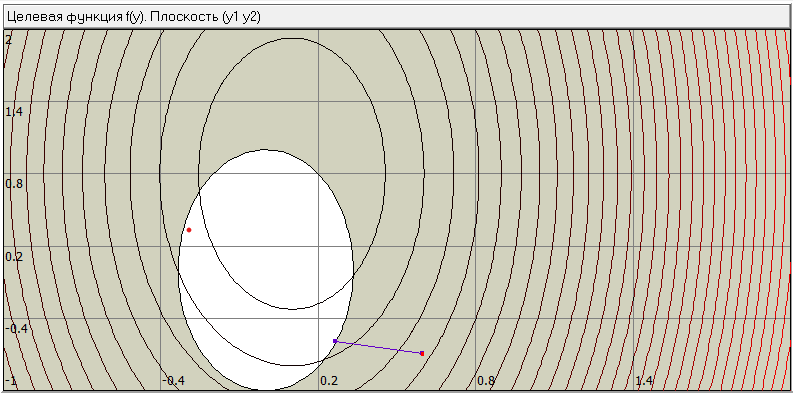
\includegraphics{05.png}
    \caption{$r = 0.5$}
\end{figure}

В случае $ r > 1 $ появляется гладкость ($r \le 2$ -- первого порядка, $r \le 3$ -- второго и т.д.) и можем спокойно использовать метод. Так при $r = 2$ наблюдаем, что метод сошёлся в точку минимума за $10$ итераций.
\begin{figure}[H]
    \centering
    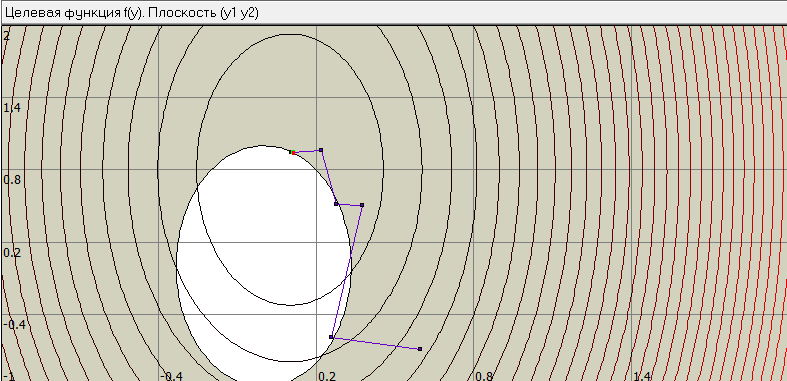
\includegraphics{2.png}
    \caption{$r = 2$}
\end{figure}

При этом для обеспечения высокой точности решения задачи значение коэффициента штрафа должно стать очень большим, но это приводит к плохой обусловленности задачи со штрафом (то есть к её сильной овражности).

Повышая значение $r$, увеличивается число итераций метода. При 
$r = 3.5$ оно становится равным $18$.
\begin{figure}[H]
    \centering
    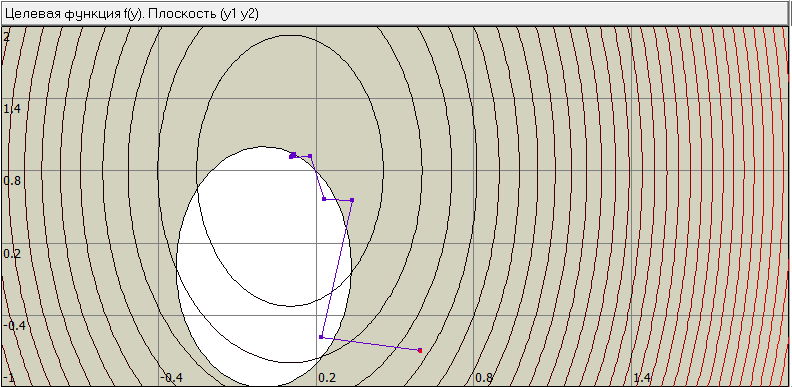
\includegraphics{35.png}
    \caption{$r = 3.5$}
\end{figure}
При $r = 5$ (макс. значение в LocOpt) будет равно $30$.
Также подход к точке происходит из области недопустимого множества. В окрестности точки производится множество операций на уточнение решения.
\begin{figure}[H]
    \centering
    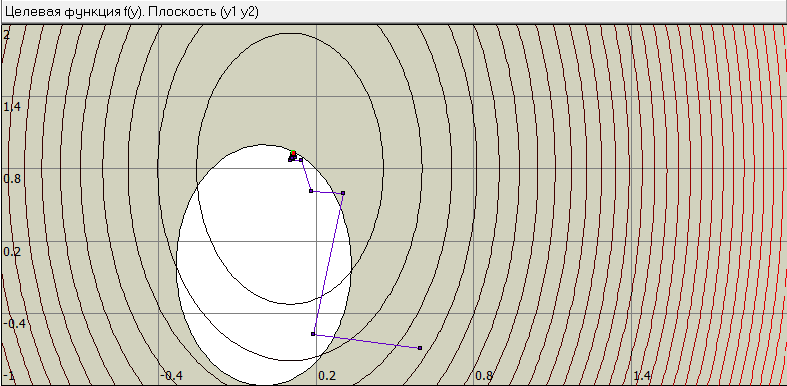
\includegraphics{5.png}
    \caption{$r = 5$}
\end{figure}

\section{Метод модифицированной функции Лагранжа}
Продемонстрируем превосходсвто метода модифицированной функции Лагранжа на той же задаче.

В методе модифицированной функции Лагранжа коэффициент штрафа $\gamma$ не обязан стремится в бесконечность, как для метода внешнего штрафа. Он должен быть достаточно большим, но конечным. Взяв $\gamma = 1000$, получим точный результ.
\begin{figure}[H]
    \centering
    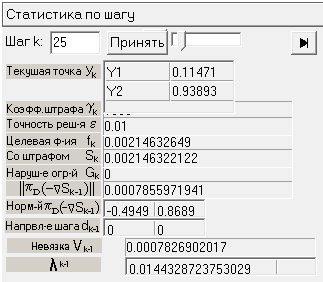
\includegraphics{lagranz.png}
\end{figure}


\end{document}